\documentclass{scrreprt}
\usepackage{listings}
\usepackage{array}
\usepackage{tikz} 
\usepackage{underscore}
\usepackage[bookmarks=true]{hyperref}
\usepackage[utf8]{inputenc}
\usepackage[english]{babel}

\usetikzlibrary{arrows.meta}
\usetikzlibrary{shapes.geometric, positioning, arrows.meta}
\usetikzlibrary{positioning}
% Define stickman style
\tikzset{
    stickman/.pic={
        % Head
        \draw[fill=gray] (0,0.6) circle (0.3cm);
        % Body
        \draw[line width=0.5mm] (0,0.3) -- (0,-0.6);
        % Arms
        \draw[line width=0.5mm] (-0.4,0.3) -- (0.4,0.3);
        % Legs
        \draw[line width=0.5mm] (0,-0.6) -- (-0.4,-1.2);
        \draw[line width=0.5mm] (0,-0.6) -- (0.4,-1.2);
},
}
\hypersetup{
    bookmarks=false,    % show bookmarks bar?
    pdftitle={Software Requirement Specification},    % title
    pdfauthor={Jean-Philippe Eisenbarth},                     % author
    pdfsubject={TeX and LaTeX},                        % subject of the document
    pdfkeywords={TeX, LaTeX, graphics, images}, % list of keywords
    colorlinks=true,       % false: boxed links; true: colored links
    linkcolor=blue,       % color of internal links
    citecolor=black,       % color of links to bibliography
    filecolor=black,        % color of file links
    urlcolor=purple,        % color of external links
    linktoc=page            % only page is linked
}
\def\myversion{1.0 }



\usepackage{hyperref}
\begin{document}


\begin{center}
    \parbox{0.8\textwidth}{ 
        \centering
        \textbf{Abstract}
    }
\end{center}

The Odyssey Travel website revolutionizes the way individuals plan and experience their journeys, providing a comprehensive platform that caters to all travel needs. Embracing the essence of convenience and personalization, Odyssey Travel offers a diverse range of travel packages, allowing users to effortlessly explore destinations and select their preferred accommodations and transportation options. The platform’s intuitive interface ensures seamless navigation, empowering users to customize their travel plans to match their unique preferences. By bridging the gap between travelers and local service providers, Odyssey Travel promotes cultural exchange and supports local economies. The website not only simplifies the travel booking process but also enhances the overall travel experience by offering tailored recommendations and insights. With a commitment to customer satisfaction and innovation, Odyssey Travel is the ultimate companion for anyone looking to embark on unforgettable adventures.


\tableofcontents
\begin{center}
    \parbox{0.8\textwidth}{ 
        \centering
        \begin{center}
            \parbox{0.8\textwidth}{ 
                \centering
                \textbf{Index of Diagrams}
            }
        \end{center}

        \begin{itemize}
            \item \textbf{Figure-5.1:} Block Diagram of Travel Agency Software \dotfill 13
            \item \textbf{Figure-5.2:} An abstract system environment of Travel Agency Software \dotfill 14
            \item \textbf{Figure-5.3:} Logical Structure of Travel Agency Software \dotfill 15
            \item \textbf{Figure-7.1:} Use Case 01 \dotfill 23
            \item \textbf{Figure-7.2:} Use Case 02 \dotfill 24
            \item \textbf{Figure-7.3:} Use Case 03 \dotfill 26
            \item \textbf{Figure-7.4:} Use Case 04 \dotfill 27
            \item \textbf{Figure-7.5:} Use Case 05 \dotfill 29
            \item \textbf{Figure-7.6:} Use Case 06 \dotfill 30
            \item \textbf{Figure-7.7:} Use Case 07 \dotfill 32
            \item \textbf{Figure-7.8:} Use Case 08 \dotfill 33
            \item \textbf{Figure-7.9:} Use Case Diagram For Travel Agency Software \dotfill 35
            \item \textbf{Figure-9.1:} Level 0 DFD of Travel Agency Software \dotfill 38
            \item \textbf{Figure-9.2:} Level 1 DFD of Travel Agency Software \dotfill 39
        \end{itemize}
        
}
\end{center}


\chapter{Overview}
{\LARGE\textbf{Preface}}
\newline
\newline
The Software Requirements Specification (SRS) provides a comprehensive outline of what the developers need to create for the system. It encompasses both user requirements and a thorough description of system specifications. This document starts with an overview of user needs, transitioning into detailed system requirements.
As an external contractor tasked with developing the system, Efficiency Monitor, we recognize the importance of this SRS in defining the technical and non-functional requirements of the software. It ensures that we don't overlook system-wide requirements while concentrating on functional aspects.
In essence, this SRS document will primarily delineate user requirements along with overarching non-functional system requirements.
\newline
\newline
{\LARGE\textbf{Readership}}
\newline
\newline
This requirements document is designed for a broad audience, including senior management, software engineers, and everyone involved in the project. Its primary audience includes customers, system analysts, project managers, designers, developers, and testers. Essentially, anyone connected to the development and maintenance of the software will refer to this document.

The SRS will be reviewed by our customers to confirm that it accurately reflects the requirements gathered from user interviews. Designers will use it as a fundamental resource for the design phase. Developers and testers will rely on this document to understand their tasks and ensure they meet the specified requirements. In summary, this document serves as a critical reference point for all stakeholders involved in the software's lifecycle.
\newline
\newline
{\LARGE\textbf{Version History}}
\newline
\newline
Since this is the introductory version of the "Odyssey Travels" application, there is no previous history or version to reference. In version 1.0 of Odyssey Travels, our goal is to meet all identified user requirements gathered through extensive study and customer interviews (as detailed in Chapter 4 of this document).
Should users encounter any limitations or shortcomings while using our product and provide feedback or request new features, we will release updated versions of Odyssey Travels. These updates will address any reported issues, incorporate requested features, or introduce enhancements based on our own assessments.




\chapter{Introduction}

\section{Purpose}
The purpose of this document is to provide a comprehensive description of the web-based project named "Odyssey Travels," developed using Next.js. It aims to outline the system’s objectives, functionalities, user interfaces, operational constraints, and how it handles external interactions. This document serves as a detailed guide for stakeholders and developers involved in the project, ensuring a clear understanding of the system’s scope and requirements. It will define how "Odyssey Travels" enhances the online travel booking experience through innovative features and responsive web interfaces.

\section{Scope}
This web-based application, "Odyssey Travels," is designed to enhance user efficiency and streamline travel planning processes. It aims to empower users by providing intuitive tools to manage and prioritize travel itineraries and bookings seamlessly. Users will no longer need to rely on traditional methods like spreadsheets or multiple websites to organize their travel plans.
"Odyssey Travels" will enable users to categorize and prioritize travel activities effortlessly, ensuring optimal utilization of their time and resources. By offering clear insights into itinerary management and suggesting efficient scheduling of activities, the application enhances user productivity while maintaining ease of use.
Specifically, the system will guide users in making informed decisions about their travel plans, suggesting ideal times for activities to maximize efficiency throughout their journey. It will help users save valuable time by centralizing booking processes and providing real-time updates on travel arrangements. Additionally, the application will assist users in optimizing their itineraries by recommending adjustments or identifying unnecessary tasks, ensuring that their travel experiences are both productive and fulfilling.
Overall, "Odyssey Travels" aims to revolutionize the travel planning experience by offering a user-friendly interface that simplifies task management and enhances productivity, thereby meeting the diverse needs of modern travelers.


\section{Organization }
This document consists of 7 chapters, each serving a distinct purpose in detailing the "Odyssey Travels" project. The following chapter, the glossary section, provides definitions for technical terms used throughout this document, aimed at enhancing readability and understanding for all stakeholders. The third section, titled User Requirement Definition, outlines the services offered to users and encompasses non-functional system requirements. This section utilizes natural language, diagrams, and other notations that are accessible and comprehensible to our customers.
Chapter 4, System Architecture, offers a high-level overview of the planned system architecture, illustrating how functions are distributed across various modules. It also highlights components that are reused within the architecture. The subsequent chapter, System Requirement Specification, delves deeper into both functional and non-functional requirements, offering detailed descriptions and specifications. Graphical system models depicting relationships between system components and their environment are included in Chapter 6, titled System Models. Chapter 7, System Evolution, outlines the core assumptions underpinning the system's design and anticipates future changes influenced by hardware advancements and evolving user needs.
Appendices containing detailed, application-specific information relevant to "Odyssey Travels" are appended after the 7th section, providing supplementary details for stakeholders and developers.

\section{References}
IEEE: IEEE Std 830-1998 IEEE Recommended Practice for Software Requirements Specifications,
IEEE Computer Society, 1998.

\chapter{Glossary}

\section{Web Framework}
Next.js – A JavaScript framework designed for building server-side rendered (SSR) React applications, developed by Vercel.

\section{Supported Devices}
Next.js application – Any web application built using Next.js. In this document, synonymous with web application developed with Next.js
\section{DFD (Data Flow Diagram)}
A graphical representation that refers the system using functions
performed in the system and data produced by these functions.
\section{Interface}
A specification of the attributes and operations associated with a software component.
The interface is used as the means of accessing the component’s functionality.
\section{Maintenance prediction}
The process in which project managers try to predict what system changes
might be proposed and what parts of the system are likely to be the most difficult to maintain.
\section{Object Model}
A model of a software system that is structured and organized as a set of object
classes and the relationships between these classes.
\section{Object-Oriented (OO) Approach}
An approach to software development where the fundamental
abstractions in the system are independent objects.


\section{Reliabity}
The ability of a system to deliver services as specified. Reliability can be specified
quantitatively as a probability of failure on demand or as the rate of occurrence of failure.
\section{Requirement, functional}
A statement of some function or feature that should be implemented in a
system.
\section{Requirement, non-functional}
A statement of a constraint or expected behavior that applies to a
system. This constraint may refer to the emergent properties of the software that is being developed
or to the development process.
\section{Sequence Diagram}
A diagram that shows the sequence of interactions required to complete some
operation. In the UML, sequence diagrams may be associated with use cases.
\section{Software Requirements Specification}
A document that completely describes all of the functions
of a proposed system and the constraints under which it must operate. For example, this document.

\section{Software Architecture}
A model of the fundamental structure and organization of a software System.

\section{Stakeholder }
Any person with an interest in the project who is not a developer.
\section{User}
Someone who interacts with the Web Browser.
\section{User Interface}
The way in which information produced by the system is displayed and the way in which system users can access system functionality.
\section{Unified Modeling Language (UML)}
A graphical language used in object-oriented development
that includes several types of system models that provide different views of a system.
\section{Use Cases}
Use cases are a requirements discovery technique that identifies the actors involved in an
interaction and names the type of interaction.

\chapter{User Requirements Definition}
This section encompasses all functional and quality requirements of the system, including non-functional requirements. It provides a comprehensive description of the system and its complete feature set. To ensure clarity and avoid misunderstandings, user requirements are articulated in natural language.
This version clarifies the purpose of the section while maintaining its original intent and focus.

\section{External Interface Requirements}
\subsection{User Interface}
\begin{itemize}
    \item \textbf{Home}:
    \begin{itemize}
        \item Serves as the main landing page.
        \item Provides an overview of offerings and services.
        \item Designed for intuitive navigation and accessibility.
    \end{itemize}
    
    \item \textbf{About}:
    \begin{itemize}
        \item Provides comprehensive project information.
        \item Includes objectives, mission statement, team members, and background details.
        \item Builds trust and transparency.
    \end{itemize}
    
    \item \textbf{Packages}:
    \begin{itemize}
        \item Users explore various travel options and service offerings.
        \item Includes detailed descriptions, pricing information, and possibly images or videos.
        \item Supports informed decision-making.
    \end{itemize}
    
    \item \textbf{Login}:
    \begin{itemize}
        \item Registered users access their accounts securely.
        \item Provides access to booking history, saved preferences, and account settings.
        \item Enhances user engagement and personalized experiences.
    \end{itemize}
    
    \item \textbf{Signup}:
    \begin{itemize}
        \item New users create accounts easily.
        \item Access to exclusive features and personalized recommendations.
        \item Facilitates seamless booking experiences.
    \end{itemize}
    
    \item \textbf{Contact Us}:
    \begin{itemize}
        \item Provides essential contact information.
        \item Includes email addresses, phone numbers, and possibly a contact form.
        \item Facilitates direct communication with customer support or the project team.
    \end{itemize}
\end{itemize}

\section*{Design Considerations}
Each section is designed with:
\begin{itemize}
    \item User-friendliness in mind.
    \item Intuitive navigation and accessibility across different devices and platforms.
    \item Home page as the focal point for engaging users.
    \item About section for building trust and transparency.
    \item Packages section for comprehensive showcasing and informed decision-making.
    \item Seamless Login and Signup process for enhanced engagement and personalized experiences.
    \item Contact Us section for easy access to customer support and inquiries.
    \item Promotion of customer satisfaction and support throughout user interaction.
\end{itemize}

\subsection*{Hardware Interfaces}
Odyssey Travels, the hardware interface consists of Android-based smartphones. There are no specific hardware requirements for the Android devices used, except that the system must be compatible with any version of Android
\section{Functional Requirements}
This section outlines the fundamental actions required for the Odyssey Travels software system:
\begin{itemize}
    \item The system must allow users to view available travel packages and details.
    \item The system must provide options to filter packages based on destination, duration, and price range.
    \item The system must display a progress bar indicating booking completion and show the percentage of bookings done.
    \item The system must offer a statistical view of popular travel destinations, package categories, and user preferences.
    \item The system must Send Invoice Mail for important booking updates and travel reminders.
    \item The system must display average user ratings and reviews for each travel package.
    \item The system must allow users to upload images or documents (e.g., passport copies) securely for booking purposes.
    \item The system must include a calendar view for users to select travel dates and check availability.
    \item The system must provide a profile section for users to manage personal information, preferences, and past bookings.
    \item The system must feature interactive travel quizzes to engage users and provide insights into destinations.
    \item The system must maintain a history of user bookings and travel preferences for personalized recommendations.
    \item All functionalities can be accessed and executed using the touchscreen interface of a smartphone.
\end{itemize}
All functionalities can be accessed and executed using the touchscreen interface of a smartphone.

\section {Non Functional Requirements}
\begin{itemize}
    \item System must provide a pleasant and user-friendly graphical interface.
    \item System must provide multilingual advantage, especially Bengali and English.
    \item System must respond within a few seconds.
    \item System must work with relatively long input lists.
    \item System mustn’t alter the task list automatically.
    \item System must restart instantly in case of failure without any data loss.
    \item System must be usable to every class of users, even if they have no technical knowledge.
    \item System must work cooperatively with other key processes without causing any delay.
\end{itemize}

\chapter {System Architecture}
This section will give an overview of the whole system. The system will be explained in its context
to show how the system interacts with user and introduce the basic functionality of it. It will also
describe what functionality is available for stakeholders. At last, the constraints and assumptions for
the system will be presented.

\section {Product perspective and functions}
Odyssey Travels is a web-based software application designed to manage travel plans and bookings efficiently. Users can seamlessly book flights, hotels, and transportation, ensuring a streamlined travel experience. The application provides tools for organizing and managing travel itineraries, allowing users to keep track of their bookings and view relevant travel details. Additional minor functions and enhancements will be detailed later in this report. In this subsection, we will present a block diagram illustrating the main functionalities of our system. The block diagram, shown in Figure 5.1, provides a visual representation of the key features and interactions within Odyssey Travels.
\newline
\newline
\begin{center}
    \parbox{0.8\textwidth}{ 
        \centering
        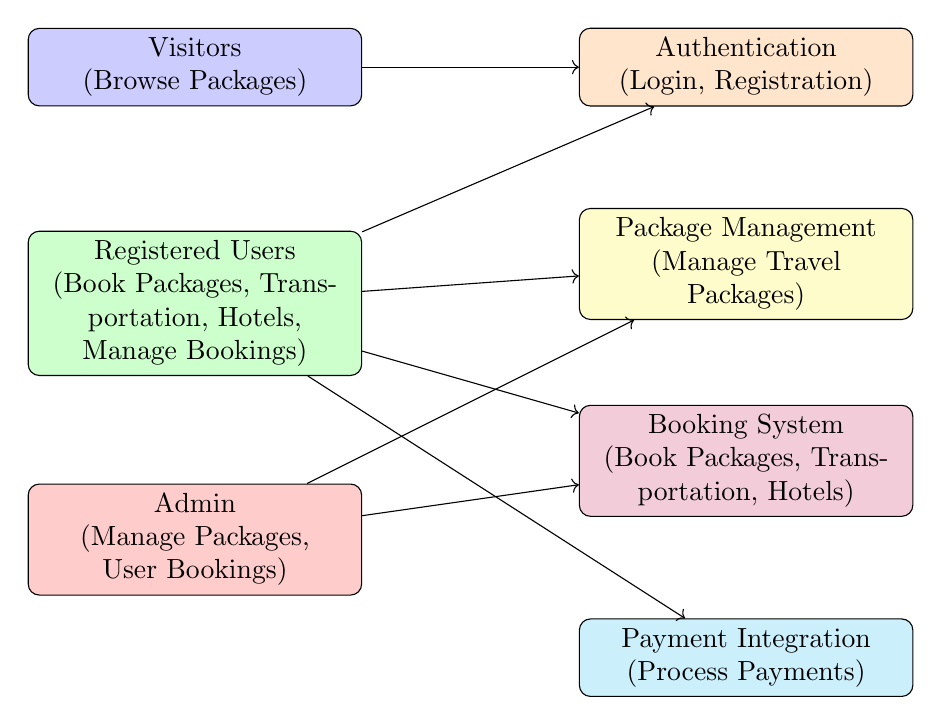
\begin{tikzpicture}[node distance=2cm, auto]
            % Define blocks
            \node [rectangle, draw, fill=blue!20, rounded corners, text centered, text width=4cm] (visitor) {Visitors \\ (Browse Packages)};
            \node [rectangle, draw, fill=green!20, rounded corners, below of=visitor, yshift=-1cm, text centered, text width=4cm] (user) {Registered Users \\ (Book Packages, Transportation, Hotels, Manage Bookings)};
            \node [rectangle, draw, fill=red!20, rounded corners, below of=user, yshift=-1cm, text centered, text width=4cm] (admin) {Admin \\ (Manage Packages, User Bookings)};
        
            \node [rectangle, draw, fill=orange!20, rounded corners, right of=visitor, xshift=5cm, text centered, text width=4cm] (auth) {Authentication \\ (Login, Registration)};
            \node [rectangle, draw, fill=yellow!20, rounded corners, below of=auth, yshift=-0.5cm, text centered, text width=4cm] (package) {Package Management \\ (Manage Travel Packages)};
            \node [rectangle, draw, fill=purple!20, rounded corners, below of=package, yshift=-0.5cm, text centered, text width=4cm] (booking) {Booking System \\ (Book Packages, Transportation, Hotels)};
            \node [rectangle, draw, fill=cyan!20, rounded corners, below of=booking, yshift=-0.5cm, text centered, text width=4cm] (payment) {Payment Integration \\ (Process Payments)};
        
            % Define arrows
            \draw [->] (visitor) -- (auth);
            \draw [->] (user) -- (auth);
            \draw [->] (user) -- (package);
            \draw [->] (user) -- (booking);
            \draw [->] (user) -- (payment);
            \draw [->] (admin) -- (package);
            \draw [->] (admin) -- (booking);
        \end{tikzpicture}
    }
\end{center}

\begin{center}
    \parbox{0.8\textwidth}{ 
        \centering
        \textbf{Figure-5.1: Block Diagram of Travel Agency Software}
    }
\end{center}

\section{System Environment}
While considering the basic functions/features of Travel Agency Software ,a sample System Environment can be imagined before analyzing the requirements in details. The abstract System Environment of our product is shown in figure-5.2 
\newline
\newline
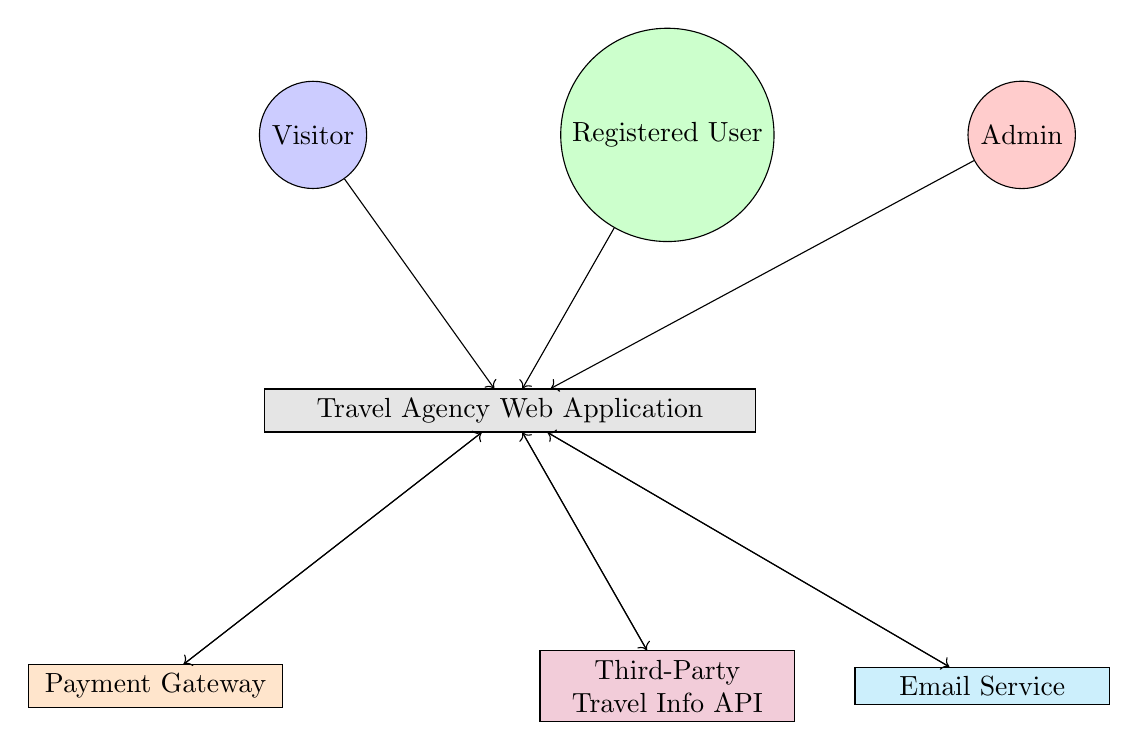
\begin{tikzpicture}[node distance=2.5cm, auto]
    % External Users
    \node [circle, draw, fill=blue!20, text centered] (visitor) {Visitor};
    \node [circle, draw, fill=green!20, right of=visitor, xshift=2cm, text centered] (user) {Registered User};
    \node [circle, draw, fill=red!20, right of=user, xshift=2cm, text centered] (admin) {Admin};
    
    % System Component
    \node [rectangle, draw, fill=gray!20, below of=visitor, xshift=2.5cm, yshift=-1cm, text centered, text width=6cm] (system) {Travel Agency Web Application};
    
    % External Systems
    \node [rectangle, draw, fill=orange!20, below of=system, xshift=-4.5cm, yshift=-1cm, text centered, text width=3cm] (payment) {Payment Gateway};
    \node [rectangle, draw, fill=purple!20, below of=system, xshift=2cm, yshift=-1cm, text centered, text width=3cm] (api) {Third-Party Travel Info API};
    \node [rectangle, draw, fill=cyan!20, below of=system, xshift=6cm, yshift=-1cm, text centered, text width=3cm] (email) {Email Service};

    % Arrows
    \draw [->] (visitor) -- (system);
    \draw [->] (user) -- (system);
    \draw [->] (admin) -- (system);
    
    \draw [->] (system) -- (payment);
    \draw [->] (system) -- (api);
    \draw [->] (system) -- (email);
    
    \draw [->] (payment) -- (system);
    \draw [->] (api) -- (system);
    \draw [->] (email) -- (system);

\end{tikzpicture}
\begin{center}
    \parbox{0.8\textwidth}{ 
        \centering
        \textbf{Figure-5.2: An abstract system environment of Travel Agency Software}
    }
\end{center}

After studying the requirements mentioned by user  listed in section 4 , we have figured out a basic logic structure of Efficiency Monitor mobile application. shown in figure-5.3. That structure basically shows the primary activities, actors, features and primary relationships between them. In general language, logic diagram shows who is doing and what is doing.


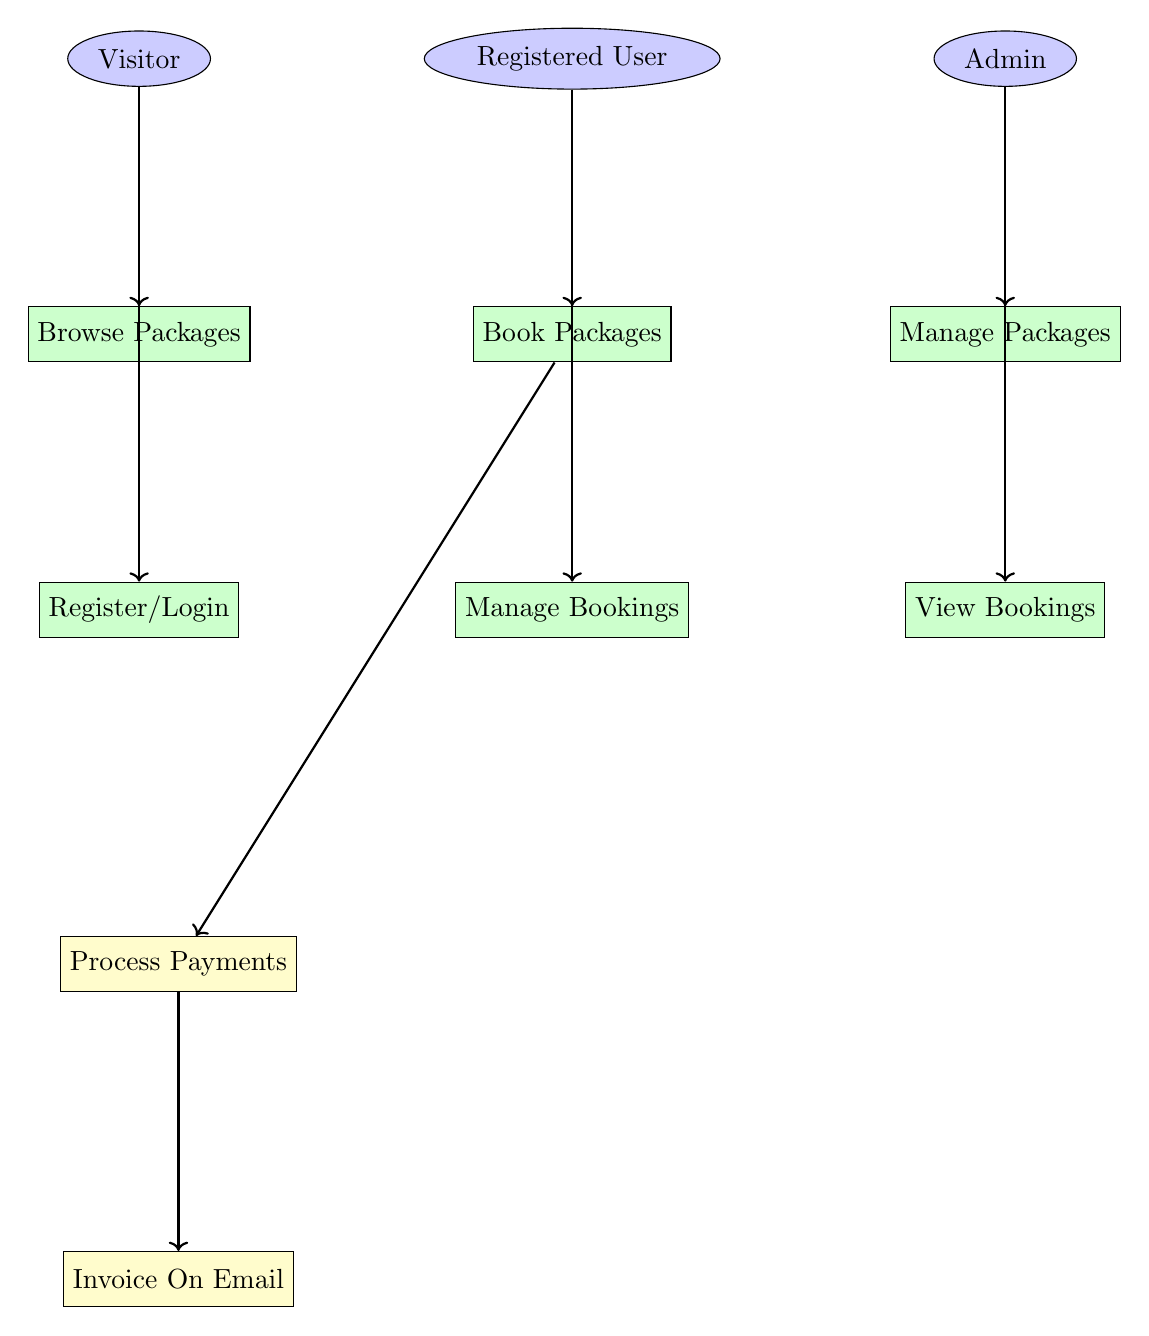
\begin{tikzpicture}[node distance=2.5cm, auto]
    % Define styles
    \tikzstyle{actor} = [ellipse, draw, fill=blue!20, text centered, minimum height=2em]
    \tikzstyle{activity} = [rectangle, draw, fill=green!20, text centered, minimum height=2em]
    \tikzstyle{feature} = [rectangle, draw, fill=yellow!20, text centered, minimum height=2em]
    \tikzstyle{relation} = [->, thick]

    % Actors
    \node[actor] (visitor) {Visitor};
    \node[actor, right of=visitor, xshift=3cm] (user) {Registered User};
    \node[actor, right of=user, xshift=3cm] (admin) {Admin};

    % Activities for Visitor
    \node[activity, below of=visitor, yshift=-1cm] (browse) {Browse Packages};
    \node[activity, below of=browse, yshift=-1cm] (register) {Register/Login};

    % Activities for Registered User
    \node[activity, below of=user, yshift=-1cm] (book) {Book Packages};
    \node[activity, below of=book, yshift=-1cm] (manageBooking) {Manage Bookings};

    % Activities for Admin
    \node[activity, below of=admin, yshift=-1cm] (managePackage) {Manage Packages};
    \node[activity, below of=managePackage, yshift=-1cm] (viewBooking) {View Bookings};

    % System Features
    \node[feature, below of=manageBooking, yshift=-2cm, xshift=-5cm] (payment) {Process Payments};
    \node[feature, below of=payment, yshift=-1.5cm] (notification) {Invoice On Email};

    % Relations
    \draw[relation] (visitor) -- (browse);
    \draw[relation] (visitor) -- (register);
    \draw[relation] (user) -- (book);
    \draw[relation] (user) -- (manageBooking);
    \draw[relation] (admin) -- (managePackage);
    \draw[relation] (admin) -- (viewBooking);

    \draw[relation] (book) -- (payment);
    \draw[relation] (payment) -- (notification);
    

\end{tikzpicture}
\begin{center}
    \parbox{0.8\textwidth}{ 
        \centering
        \textbf{Figure-5.3:Logical Structure of Travel Agency Software}
    }
\end{center}

\section {User characteristics}
There is a single type of user interacting with the system: users of the Odyssey Travels web application. Users of our web app have specialized usage tailored to their travel planning and booking needs.
The web application allows users to explore travel packages, manage their travel itineraries, and modify their bookings at any time. This means that users need to be able to view available packages, add new bookings, and update their travel plans seamlessly.
For optimal use of our solution, users are expected to be familiar with basic web navigation and interaction. This includes the ability to use buttons, dropdown menus, side panels, and other common web interface elements effectively.
\section{Assumptions and dependencies}
One assumption about the Odyssey Travels application is that it will be used on mobile devices with adequate performance capabilities. If the device lacks sufficient hardware resources, such as processing power, RAM, or storage space, or if these resources are heavily utilized by other applications, the performance of Odyssey Travels may be compromised. In such cases, users may experience issues where the application does not function as intended, or may not work at all.


\chapter{System Requirement Specification}
Under this headline we’ll describe all the functional and non-functional requirements in details.

\section{External Interface Requirements}
This subsection provides a comprehensive description of all user interface requirements for the Odyssey Travels system. It also includes detailed descriptions of the software interfaces involved in the system's operation.
\subsection{User Interfaces – GUI}
The primary elements of Odyssey Travels' GUI are:

\begin{itemize}
    \item \textbf{Home Page}:
    \begin{itemize}
        \item Main landing page with navigation to sections such as 'About,' 'Packages,' 'Login,' 'Signup,' and 'Contact Us.'
        \item Title bar includes a navigation menu, application logo, and quick access to notifications and user profile.
    \end{itemize}
    
    \item \textbf{Packages Page}:
    \begin{itemize}
        \item Displays available travel packages with options to filter and sort based on destination, duration, price, etc.
        \item Detailed descriptions, images, and booking options for each package.
        \item Users can select packages to view more details or proceed to booking.
    \end{itemize}
    
    \item \textbf{Login and Signup Pages}:
    \begin{itemize}
        \item 'Login' page for existing users to enter credentials and access their accounts.
        \item 'Signup' page for new users to create accounts by providing name, email, and password.
        \item Both pages support secure authentication and password recovery.
    \end{itemize}
    
    \item \textbf{About Page}:
    \begin{itemize}
        \item Provides insights into the project’s mission, team, and background information.
        \item Helps users understand Odyssey Travels' goals and the team behind it.
    \end{itemize}
    
    \item \textbf{Contact Us Page}:
    \begin{itemize}
        \item Contains contact information, an inquiry form, and links to support resources.
        \item Facilitates direct communication with the Odyssey Travels team.
    \end{itemize}
    
    \item \textbf{Profile Page}:
    \begin{itemize}
        \item Accessible from the user icon on the Home page.
        \item Options to view and edit personal details, change profile picture, and review booking history.
        \item Enables convenient management of user profiles.
    \end{itemize}
    
    \item \textbf{Invoices:}:
    \begin{itemize}
        \item Invoices for selected travel packages are automatically emailed to users.
        \item  Each email contains a detailed breakdown of the booking, including costs, services, and travel itinerary.
        \item Ensures users receive timely and accurate information about their purchases and can easily access their invoices for record-keeping.
    \end{itemize}
    \item \textbf{Interactive Features}:
    \begin{itemize}
        \item Home page includes interactive elements like travel quizzes and engagement activities.
        \item Enhances user experience with fun exploration of travel-related content and rewards or insights.
    \end{itemize}
    
\end{itemize}

\subsection{Hardware and software interfaces}
Odyssey Travels is a mobile-friendly web application for travel planning and booking, accessible via Android (7.0+) and iOS (11.0+) devices using modern web browsers. It supports touch gestures and requires a minimum screen resolution of 720 x 1280 pixels. Push notifications keep users updated on booking details and promotions in real-time.
Backend services utilize RESTful APIs for data retrieval and storage of user profiles, travel packages, and bookings, with secure authentication and payment gateways like PayPal and Stripe. Mapping services such as Google Maps or Mapbox provide location and direction functionalities.
JavaScript frameworks like React and Next.js optimize frontend functionality, while Axios manages HTTP requests. Cloud storage ensures secure management of user-uploaded documents and images, and email services handle communication with users. Overall, Odyssey Travels maximizes usability and efficiency through its robust hardware and software interfaces for travel planning and booking on mobile devices.

\subsection{Communications interfaces}
Odyssey Travels utilizes HTTP/HTTPS protocols for secure data exchange between clients and servers, ensuring encrypted communication for user interactions and sensitive information. RESTful APIs facilitate seamless integration with backend services, enabling efficient retrieval of travel package data, user profiles, and booking details. Authentication services like OAuth or JWT manage secure user access and session handling, ensuring only authorized interactions within the application. Payment gateways such as PayPal and Stripe handle secure transactions, complying with PCI DSS standards for payment security. SMTP or Email APIs (e.g., SendGrid) manage transactional emails for booking confirmations and notifications, ensuring reliable communication with users. Push notification services (e.g., Firebase Cloud Messaging) deliver real-time alerts on booking updates and promotions, enhancing user engagement. Mapping APIs (e.g., Google Maps, Mapbox) provide location-based services for travel destinations and directions, enhancing the overall travel planning experience within Odyssey Travels.

\section {Functional Requirements}
\begin{itemize}
    \item User Authentication and Profile Management: Secure registration, login, and profile management including personal details and preferences.
    \item Travel Package Browsing and Booking: Browse packages, view details (destinations, itineraries, pricing), and book securely.
    \item Notification System: Notify users about booking confirmations, package updates, and offers via push notifications and emails.
    \item Search and Filtering: Search packages by destination, duration, price range, and travel dates, with filtering options for tailored results.
    \item Payment Gateway Integration: Integrate with secure payment gateways for credit/debit card and other payment methods.
    \item User Feedback and Reviews: Provide feedback and reviews on travel experiences and interact with other users' reviews.
    \item Admin Dashboard: Manage travel packages, user accounts, and monitor booking transactions with an administrative dashboard.
\end{itemize}

These requirements ensure a user-friendly and comprehensive travel planning and booking experience for users of Odyssey Travels.

\begin{itemize}
    \item \textbf{User Registration and Authentication}
    \begin{itemize}
        \item 1.1. Users can create a new account or log in using existing credentials to access personalized features.
        \item 1.2. The system securely stores user information, including name, contact details, and login credentials.
        \item 1.3. User authentication ensures secure access to sensitive information such as booking history and payment details.
    \end{itemize}
    
    \item \textbf{Travel Package Management}
    \begin{itemize}
        \item 2.1. The system presents a catalog of travel packages categorized by destination, type (e.g., adventure, cultural), and duration.
        \item 2.2. Users can view detailed descriptions, itineraries, inclusions, and exclusions for each package.
        \item 2.3. The system allows users to filter packages by price range, departure dates, and specific amenities.
        \item 2.4. Users can add packages to a wishlist or compare multiple packages side by side for informed decision-making.
    \end{itemize}
    
    \item \textbf{Booking and Reservation System}
    \begin{itemize}
        \item 3.1. Users initiate bookings by selecting preferred travel packages and specifying travel dates.
        \item 3.2. The system calculates total costs, including taxes and additional fees, and displays payment options.
        \item 3.3. Users can choose payment methods (e.g., credit card, PayPal) and complete transactions securely.
        \item 3.4. Confirmation emails are sent to users upon successful booking, containing booking details and itinerary information.
    \end{itemize}
    
    \item \textbf{User Profile Management}
    \begin{itemize}
        \item 4.1. Users have access to a profile dashboard where they can view and manage personal information.
        \item 4.2. The system allows users to update profile details, such as contact information, travel preferences, and loyalty program memberships.
        \item 4.3. Users can upload and manage profile photos or avatars to personalize their accounts.
        \item 4.4. Profile settings include privacy options to control visibility of personal details and preferences.
    \end{itemize}
    
    \item \textbf{Notifications and Alerts}
    \begin{itemize}
        \item 5.1. The system sends real-time notifications to users regarding booking confirmations, itinerary changes, and special promotions.
        \item 5.2. Users can customize notification preferences based on their interests and travel plans.
        \item 5.3. Alerts include reminders for upcoming trips, payment due dates, and recommendations for additional services.
    \end{itemize}
    
    \item \textbf{Interactive Maps and Location Services}
    \begin{itemize}
        \item 6.1. Integrated mapping APIs provide interactive maps displaying travel destinations, nearby attractions, and points of interest.
        \item 6.2. Users can search for specific locations, view directions, and explore interactive maps with zoom and pan functionalities.
        \item 6.3. The system offers offline access to maps and travel guides, ensuring usability even in areas with limited connectivity.
    \end{itemize}
    
    \item \textbf{Customer Support and Feedback}
    \begin{itemize}
        \item 7.1. Users access customer support options through the application, including FAQs, help guides, and contact forms.
        \item 7.2. The system facilitates live chat support for immediate assistance with booking inquiries and technical issues.
        \item 7.3. Users can submit feedback and reviews about their travel experiences, helping to improve service quality and user satisfaction.
    \end{itemize}
    
    \item \textbf{Language and Accessibility Options}
    \begin{itemize}
        \item 8.1. The application supports multiple languages, allowing users to select their preferred language for navigation and communication.
        \item 8.2. Accessibility features ensure that the application is usable by users with disabilities, including screen readers and text-to-speech capabilities.
    \end{itemize}
    
    \item \textbf{System Security and Data Privacy}
    \begin{itemize}
        \item 9.1. The system employs encryption protocols (e.g., HTTPS) to secure data transmission and protect user information.
        \item 9.2. User data, including personal details and payment information, is stored securely and compliant with data protection regulations.
        \item 9.3. Regular security audits and updates are conducted to maintain the integrity and confidentiality of user data.
    \end{itemize}
\end{itemize}

\section{Non Functional Requirements}
Odyssey Travels prioritizes performance with a goal of rapid response times and seamless transaction handling for up to 1000 concurrent users. It ensures high reliability through robust error handling and data recovery mechanisms, aiming for 99.9% uptime. Security measures include encryption of user data, strict access controls, and regular security audits.
Scalability is addressed with a horizontally scalable infrastructure to accommodate peak traffic and increasing user volumes. Usability focuses on an intuitive interface across devices, employing responsive design principles. Compatibility is assured across major web browsers and mobile platforms (Android, iOS), ensuring consistent functionality and user experience.

Maintainability is facilitated through best coding practices and comprehensive documentation, supporting efficient system management and future enhancements. These non-functional requirements collectively ensure a secure, scalable, and user-centric travel booking experience with Odyssey Travels.

\subsection{Performance Requirements}
Odyssey Travels is an application that operates efficiently without imposing significant demands on system resources, ensuring minimal impact on other essential processes. It is designed to deliver prompt responses, providing users with a real-time experience for seamless interaction and efficient service delivery.

\subsection {Safety Requirements}
The Odyssey Travels application guarantees the integrity of user-inputted data, ensuring no alterations to these entries. It is designed to operate reliably even with extensive task lists and under various configuration settings, maintaining functionality and performance without compromise.

\subsection {Software Quality Attribute}
Odyssey Travels offers a user-friendly graphical interface designed for ease of use, featuring straightforward functionalities. Users of all levels should navigate the application effortlessly, requiring no specialized knowledge. The system prioritizes quick responsiveness to ensure a seamless user experience
\subsection {Reliability}
The system must be reliable to users. In case of system failure it must restart instantly without anydata loss.
\subsection {Multi lingual Support}
The system should be language agnostic. English and Bengali should be at least be supported
because these are the the native languages of users.



\chapter{System Models}
In this chapter, we will construct abstract models of the system to depict various views or perspectives using predefined graphical notations, particularly the Unified Modeling Language (UML). System modeling serves to elucidate the intended requirements to stakeholders, facilitating discussions on design proposals and providing comprehensive documentation for implementation. This section includes subsections detailing use cases and essential diagrams that illustrate the functionality and structure of our system.

\section{Use Cases}
Use Cases help us to identify the actors involved in an interaction and names the type of interaction.
This subsection outlines the Use Cases for our system’s users. Use cases are determined following
the scenarios mentioned in section-6.

\section*{\textbf{7.1.1. UC 1: Users Viewing Packages}}
\textbf{Diagram:}
\newline
\newline
\begin{center}
    \parbox{0.8\textwidth}{ 
        \centering
        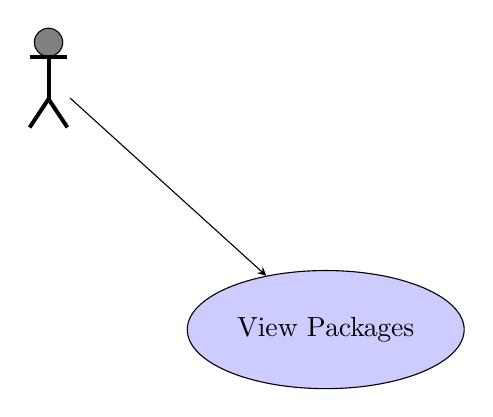
\begin{tikzpicture}[>=stealth]

            % Actor (stickman)
            \node[inner sep=0pt] (user) at (0,0) {\tikz{\pic[scale=0.6] {stickman};}};
        
            % Use Case with color
            \node[ellipse, draw, fill=blue!20, align=center, minimum width=3cm, minimum height=1.5cm, below right=2cm and 2cm of user] (view) {View Packages};
        
            % Relationships
            \draw[->] (user) -- (view);
        
        \end{tikzpicture}
    }
\end{center}

\begin{center}
    \parbox{0.8\textwidth}{ 
        \centering
        \textbf{Figure-7.1: Use Case 01}
    }
\end{center}

\paragraph {\textnormal{Brief Description: 
Users view available travel packages on the Odyssey Travels platform.}}

\textbf{Preconditions:}
\begin{itemize}
    \item User has a working internet connection.
    \item Odyssey Travels application is installed on the device.
\end{itemize}

\textbf{Main Success Scenario:}
\begin{enumerate}
    \item User opens the Odyssey Travels application.
    \item System displays the home screen with navigation options: Home, About, Packages, Login, Signup, Contact Us.
    \item User taps on the "Packages" option from the navigation menu.
    \item System shows the "Packages" page, listing various travel packages available.
    \item User scrolls through the list of packages to explore details and options.
    \item System displays package details including destination, duration, pricing, and amenities.
    \item User selects a specific package for more detailed information.
    \item System shows detailed information such as itinerary, inclusions, and exclusions.
    \item User navigates back to the package list or other sections using navigation buttons.
\end{enumerate}

\textbf{Postcondition:}
\begin{itemize}
    \item System displays the selected package details accurately.
    \item User can proceed to book the selected package or explore other options.
\end{itemize}

\section*{\textbf{7.1.2. UC 2: Purchase Plan}}
\textbf{Diagram:}
\newline
\newline
\begin{center}
    \parbox{0.8\textwidth}{ 
        \centering
        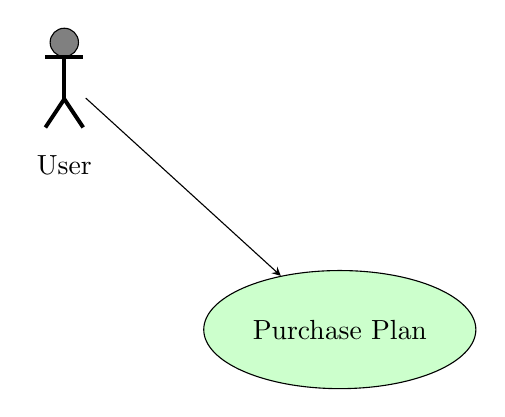
\begin{tikzpicture}[>=stealth]

            % Actor (stickman)
            \node[inner sep=0pt] (user) at (0,0) {\tikz{\pic[scale=0.6] {stickman};}};
            \node[below=0.2cm of user] {User};
        
            % Use Case with color
            \node[ellipse, draw, fill=green!20, align=center, minimum width=3cm, minimum height=1.5cm, below right=2cm and 2cm of user] (purchase) {Purchase Plan};
        
            % Relationships
            \draw[->] (user) -- (purchase);
        
        \end{tikzpicture}
    }
\end{center}

\begin{center}
    \parbox{0.8\textwidth}{ 
        \centering
        \textbf{Figure-7.2: Use Case 02}
    }
\end{center}
\paragraph {\textnormal{Brief Description: 
User selects and purchases a travel plan on the Odyssey Travels platform.\newline
}}
\textbf{Preconditions:}
\begin{itemize}
    \item User has a working internet connection.
    \item Odyssey Travels application is installed on the device.
    \item User is logged into the Odyssey Travels account.
\end{itemize}

\textbf{Main Success Scenario:}
\begin{enumerate}
    \item System displays the home page of the Odyssey Travels application.
    \item User navigates to the "Packages" section from the navigation menu.
    \item System shows a list of available travel packages.
    \item User selects a specific travel package for purchase.
    \item System displays detailed information about the selected package, including itinerary, pricing, and booking options.
    \item User confirms the package selection and taps on the "Book Now" button.
    \item System prompts the user to enter necessary details such as travel dates, number of travelers, and any additional preferences.
    \item User fills in the required information and proceeds to the payment section.
    \item System securely processes the payment using the chosen payment method (e.g., credit card, PayPal).
    \item System confirms the successful booking and displays a confirmation message with booking details.
    \item User receives a confirmation email with the booking details.
\end{enumerate}

\textbf{Postconditions:}
\begin{itemize}
    \item User's selected travel plan is successfully booked and confirmed.
    \item System displays the home page or booking summary for the user to review.
\end{itemize}

\textbf{Alternative Courses:}
\begin{itemize}
    \item[5a.] User explores additional details or options before making a final selection.
    \item[7a.] User adjusts travel details or preferences before confirming the booking.
    \item[9a.] Payment transaction fails or encounters issues; system prompts user to retry or choose an alternative payment method.
\end{itemize}

\textbf{Exceptions:}
\begin{itemize}
    \item User may abandon the booking process at any step before final confirmation.
\end{itemize}

\section*{\textbf{7.1.3. UC 3: Purchase Plan with Apply Coupon}}
\textbf{Diagram:}
\newline
\newline
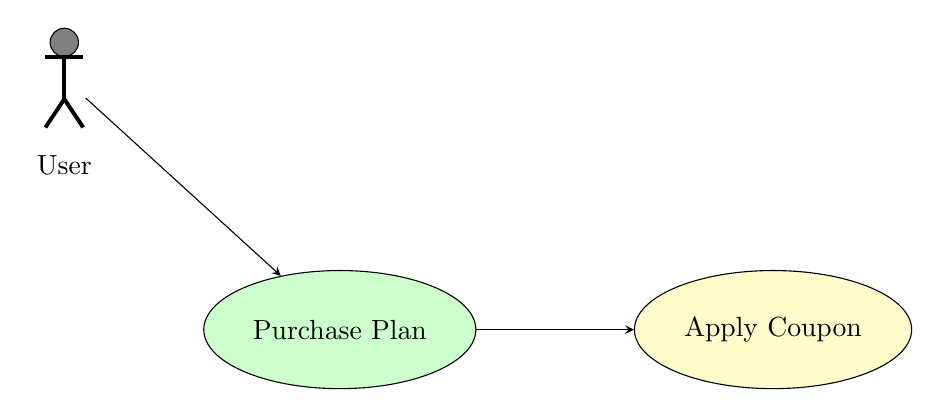
\begin{tikzpicture}[>=stealth]

    % Actor (stickman)
    \node[inner sep=0pt] (user) at (0,0) {\tikz{\pic[scale=0.6] {stickman};}};
    \node[below=0.2cm of user] {User};

    % Use Cases with color
    \node[ellipse, draw, fill=green!20, align=center, minimum width=3cm, minimum height=1.5cm, below right=2cm and 2cm of user] (purchase) {Purchase Plan};
    \node[ellipse, draw, fill=yellow!20, align=center, minimum width=3cm, minimum height=1.5cm, right=2cm of purchase] (apply) {Apply Coupon};

    % Relationships
    \draw[->] (user) -- (purchase);
    \draw[->] (purchase) -- (apply);

\end{tikzpicture}
\begin{center}
    \parbox{0.8\textwidth}{ 
        \centering
        \textbf{Figure-7.3: Use Case 03}
    }
\end{center}


\paragraph {\textnormal{Brief Description: 
User applies a coupon code during the booking process to avail discounts or special offers.}}

\subsection*{\textbf{UC 3: Apply Coupon}}

\textbf{Preconditions:}
\begin{itemize}
    \item User has a working internet connection.
    \item Odyssey Travels application is installed on the device.
    \item User is logged into the Odyssey Travels account.
    \item User has selected a travel package and proceeded to the payment section.
\end{itemize}

\textbf{Main Success Scenario:}
\begin{enumerate}
    \item System displays the booking details and prompts the user to apply a coupon code.
    \item User enters the coupon code in the designated field.
    \item System verifies the coupon validity and applies the discount to the total booking amount.
    \item System updates the payment summary to reflect the discounted price.
    \item User confirms the application of the coupon code.
    \item System confirms the coupon code application and adjusts the total payable amount accordingly.
\end{enumerate}

\textbf{Postconditions:}
\begin{itemize}
    \item System displays the updated booking summary with the discounted price.
    \item User proceeds to complete the booking with the discounted price.
\end{itemize}

\textbf{Alternative Courses:}
\begin{itemize}
    \item[3a.] User enters an invalid coupon code or expired coupon.
    \begin{itemize}
        \item[3a.01.] System displays an error message indicating the issue with the coupon code.
        \item[3a.02.] User can retry with a different coupon code or proceed without applying any coupon.
    \end{itemize}
\end{itemize}

\textbf{Exceptions:}
\begin{itemize}
    \item User may abandon the coupon application process at any step before confirmation.
\end{itemize}


\section*{\textbf{7.1.4. UC 4: Book Flight and Transportation}}


\textbf{Diagram:}
\newline
\newline
\begin{center}
    \parbox{0.8\textwidth}{ 
        \centering
        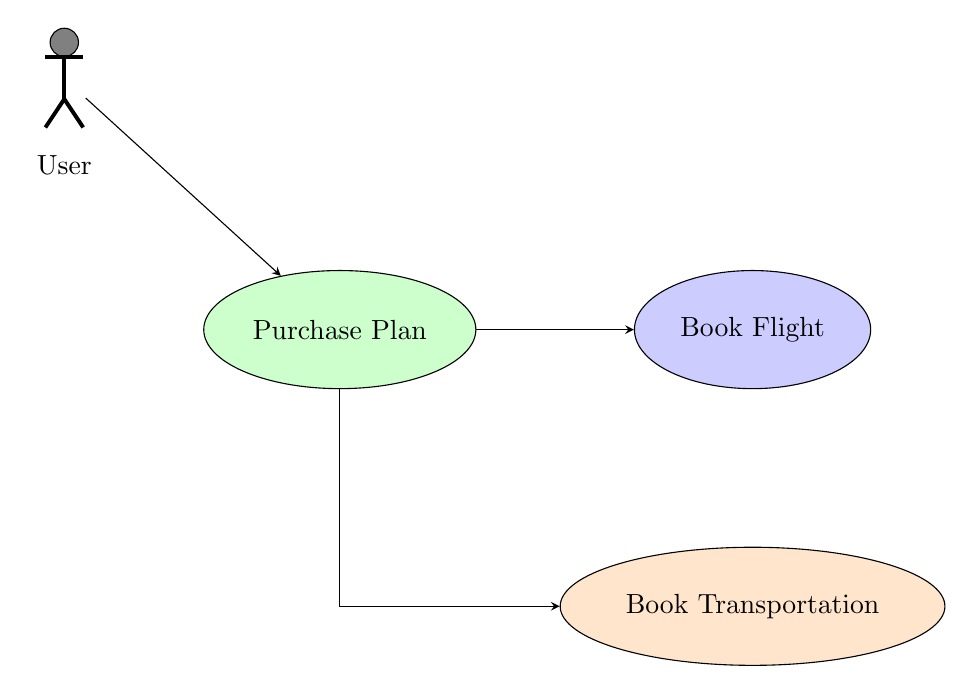
\begin{tikzpicture}[>=stealth]

            % Actor (stickman)
            \node[inner sep=0pt] (user) at (0,0) {\tikz{\pic[scale=0.6] {stickman};}};
            \node[below=0.2cm of user] {User};
        
            % Use Cases with color
            \node[ellipse, draw, fill=green!20, align=center, minimum width=3cm, minimum height=1.5cm, below right=2cm and 2cm of user] (purchase) {Purchase Plan};
            \node[ellipse, draw, fill=blue!20, align=center, minimum width=3cm, minimum height=1.5cm, right=2cm of purchase] (flight) {Book Flight};
            \node[ellipse, draw, fill=orange!20, align=center, minimum width=3cm, minimum height=1.5cm, below=2cm of flight] (transportation) {Book Transportation};
        
            % Relationships
            \draw[->] (user) -- (purchase);
            \draw[->] (purchase) -- (flight);
            \draw[->] (purchase) |- (transportation);
        
        \end{tikzpicture}
    }
\end{center}
\begin{center}
    \parbox{0.8\textwidth}{ 
        \centering
        \textbf{Figure-7.4: Use Case 04}
    }
\end{center}
\paragraph {\textnormal{Brief Description: 
User selects and books flights and transportation services through the Odyssey Travels application.}}


\subsection*{\textbf{UC 4: Book Flight and Transportation}}

\textbf{Preconditions:}
\begin{itemize}
    \item User has a working internet connection.
    \item Odyssey Travels application is installed on the device.
    \item User is logged into the Odyssey Travels account.
    \item User has navigated to the booking section of the app.
\end{itemize}

\textbf{Main Success Scenario:}
\begin{enumerate}
    \item System displays the home page of the Odyssey Travels App.
    \item User taps on the 'Book Flight and Transportation' option from the display screen.
    \item System displays a list of available flights and transportation options.
    \item User selects a flight and transportation option.
    \item System prompts user to enter travel details such as departure date, return date, number of passengers, etc.
    \item User fills in the required details.
    \item System calculates the total fare and displays the payment summary.
    \item User confirms the booking details.
    \item System processes the payment transaction securely.
    \item System confirms the booking with a booking ID and sends a confirmation email or notification to the user.
    \item User receives the booking confirmation and can view the booking details in the app.
\end{enumerate}

\textbf{Postconditions:}
\begin{itemize}
    \item System updates the user's booking history with the new booking details.
    \item User can access the booked flight and transportation details under their account.
\end{itemize}

\textbf{Alternative Courses:}
\begin{itemize}
    \item[5a.] User searches for a specific flight or transportation option not listed.
    \begin{itemize}
        \item[5a.01.] System displays a message indicating no results found.
        \item[5a.02.] User can retry with different search criteria or contact support.
    \end{itemize}
\end{itemize}

\textbf{Exceptions:}
\begin{itemize}
    \item User may abandon the booking process at any step before confirming the payment.
\end{itemize}



\section*{\textbf{7.1.5. UC 5: Book Hotel}}


\textbf{Diagram:}
\newline
\newline
\begin{center}
    \parbox{0.8\textwidth}{ 
        \centering
        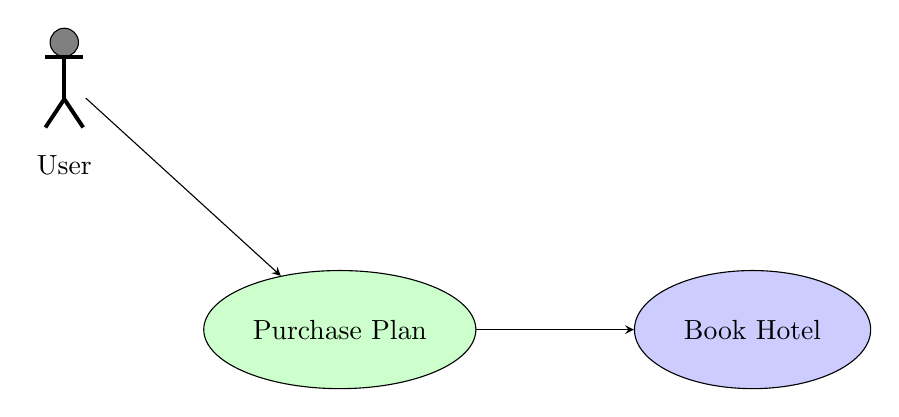
\begin{tikzpicture}[>=stealth]

            % Actor (stickman)
            \node[inner sep=0pt] (user) at (0,0) {\tikz{\pic[scale=0.6] {stickman};}};
            \node[below=0.2cm of user] {User};
        
            % Use Cases with color
            \node[ellipse, draw, fill=green!20, align=center, minimum width=3cm, minimum height=1.5cm, below right=2cm and 2cm of user] (purchase) {Purchase Plan};
            \node[ellipse, draw, fill=blue!20, align=center, minimum width=3cm, minimum height=1.5cm, right=2cm of purchase] (hotel) {Book Hotel};
        
            % Relationships
            \draw[->] (user) -- (purchase);
            \draw[->] (purchase) -- (hotel);
        
        \end{tikzpicture}
    }
\end{center}
\begin{center}
    \parbox{0.8\textwidth}{ 
        \centering
        \textbf{Figure-7.5: Use Case 05}
    }
\end{center}

\paragraph {\textnormal{Brief Description: 
User selects and books accommodations through the Odyssey Travels application.}}


\subsection*{\textbf{UC 5: Book Hotel}}

\textbf{Preconditions:}
\begin{itemize}
    \item User has a working internet connection.
    \item Odyssey Travels application is installed on the device.
    \item User is logged into the Odyssey Travels account.
    \item User has navigated to the hotel booking section of the app.
\end{itemize}

\textbf{Main Success Scenario:}
\begin{enumerate}
    \item System displays the home page of the Odyssey Travels App.
    \item User taps on the 'Book Hotel' option from the display screen.
    \item System displays a list of available hotels based on the user's search criteria.
    \item User selects a hotel from the list.
    \item System prompts user to enter details such as check-in date, check-out date, number of rooms, etc.
    \item User fills in the required details.
    \item System calculates the total cost and displays the payment summary.
    \item User confirms the booking details.
    \item System processes the payment transaction securely.
    \item System confirms the hotel booking with a booking ID and sends a confirmation email or notification to the user.
    \item User receives the booking confirmation and can view the booking details in the app.
\end{enumerate}

\textbf{Postconditions:}
\begin{itemize}
    \item System updates the user's booking history with the new hotel booking details.
    \item User can access the booked hotel details under their account.
\end{itemize}

\textbf{Alternative Courses:}
\begin{itemize}
    \item[5a.] User searches for a specific hotel not listed.
    \begin{itemize}
        \item[5a.01.] System displays a message indicating no results found.
        \item[5a.02.] User can retry with different search criteria or contact support.
    \end{itemize}
\end{itemize}

\textbf{Exceptions:}
\begin{itemize}
    \item User may abandon the booking process at any step before confirming the payment.
\end{itemize}


\section*{\textbf{7.1.6. UC 6: Admin View and Accept/Delete Plans}}
\textbf{Diagram:}
\newline
\newline

\begin{center}
    \parbox{0.8\textwidth}{ 
        \centering
       
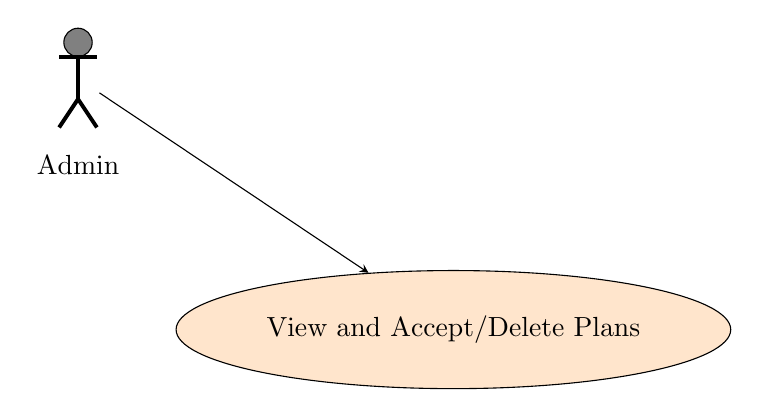
\begin{tikzpicture}[>=stealth]

    % Actor (Admin)
    \node[inner sep=0pt] (admin) at (0,0) {\tikz{\pic[scale=0.6] {stickman};}};
    \node[below=0.2cm of admin] {Admin};

    % Use Case with color
    \node[ellipse, draw, fill=orange!20, align=center, minimum width=4cm, minimum height=1.5cm, below right=2cm and 2cm of admin] (view) {View and Accept/Delete Plans};

    % Relationships
    \draw[->] (admin) -- (view);

\end{tikzpicture}
    }
\end{center}
\begin{center}
    \parbox{0.8\textwidth}{ 
        \centering
        \textbf{Figure-7.6: Use Case 06}
    }
\end{center}

\paragraph {\textnormal{Brief Description: 
Admin reviews and manages travel plans submitted by users, either accepting or deleting them based on predefined criteria.}}


\subsection*{\textbf{Main Success Scenario:}}

\begin{enumerate}
    \item \textbf{Admin logs into the Odyssey Travels admin panel.}
    \item Navigates to "Manage Travel Plans" section.
    \item Views list of submitted plans.
    \item Selects a plan for detailed review.
    \item Reviews plan details (itinerary, user info, pricing).
    \item Evaluates plan against criteria.
    \item Accepts plan: updates status, notifies user.
    \item Deletes plan: removes from system, notifies user.
    \item Records decision and notes.
\end{enumerate}

\subsection*{\textbf{Postconditions:}}

\begin{itemize}
    \item Plan status updated in database.
    \item User notified of plan status.
\end{itemize}

\subsection*{\textbf{Alternative Courses:}}

\begin{itemize}
    \item Requests additional info or corrections from user.
    \item Communicates via internal messaging or email.
\end{itemize}

\subsection*{\textbf{Exceptions:}}

\begin{itemize}
    \item Technical issues hindering plan access.
    \item Admin postpones review.
\end{itemize}

\section*{\textbf{7.1.7. UC 7: Admin View and Edit Booked Hotels of Users}}
\textbf{Diagram:}
\newline
\newline

\begin{center}
    \parbox{0.8\textwidth}{ 
        \centering
        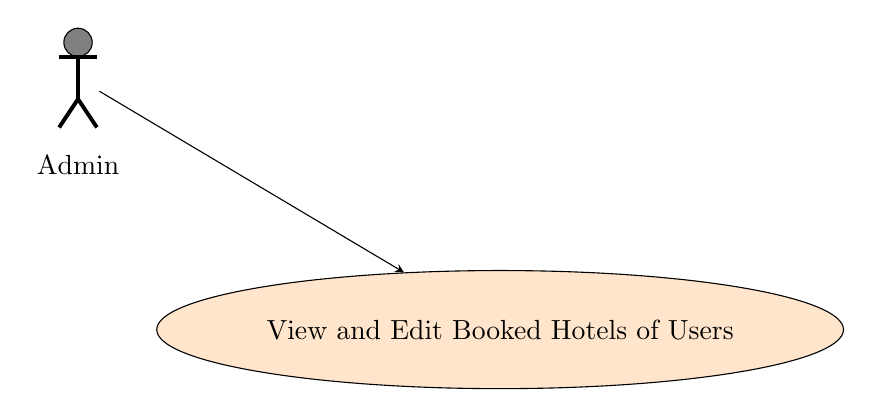
\begin{tikzpicture}[>=stealth]
            % Actor (Admin)
            \node[inner sep=0pt] (admin) at (0,0) {\tikz{\pic[scale=0.6] {stickman};}};
            \node[below=0.2cm of admin] {Admin};
        
            % Use Case with color
            \node[ellipse, draw, fill=orange!20, align=center, minimum width=6cm, minimum height=1.5cm, below right=2cm and 2cm of admin] (view) {View and Edit Booked Hotels of Users};
        
            % Relationships
            \draw[->] (admin) -- (view);
        
        \end{tikzpicture}
    }
\end{center}
\begin{center}
    \parbox{0.8\textwidth}{ 
        \centering
        \textbf{Figure-7.7: Use Case 07}
    }
\end{center}

\paragraph {\textnormal{Brief Description: 
Admin accesses and modifies hotel bookings made by users through the Odyssey Travels platform.}}

\subsection*{\textbf{Main Success Scenario:}}

\begin{enumerate}
    \item Admin logs into the Odyssey Travels admin dashboard.
    \item Navigates to "Manage Booked Hotels" section.
    \item Views list of booked hotels with user details.
    \item Selects a booked hotel for editing.
    \item Reviews booking details (dates, rooms, preferences).
    \item Edits booking information as required.
    \item Confirms changes and updates the booking.
    \item Notifies user of any modifications.
\end{enumerate}

\subsection*{\textbf{Postconditions:}}

\begin{itemize}
    \item Booking details updated in the system.
    \item User notified of changes made.
\end{itemize}

\subsection*{\textbf{Alternative Courses:}}

\begin{itemize}
    \item Requests additional information or clarifications from the user.
    \item Provides support or resolves issues related to the booking.
\end{itemize}

\subsection*{\textbf{Exceptions:}}

\begin{itemize}
    \item System downtime affecting access to bookings.
    \item Admin defers editing due to unforeseen circumstances.
\end{itemize}

\section*{\textbf{7.1.8. UC 8: Admin View, Edit, Delete Registered Tour Guide's Information}}
\textbf{Diagram:}
\newline

\begin{center}
    \parbox{0.8\textwidth}{ 
        \centering
        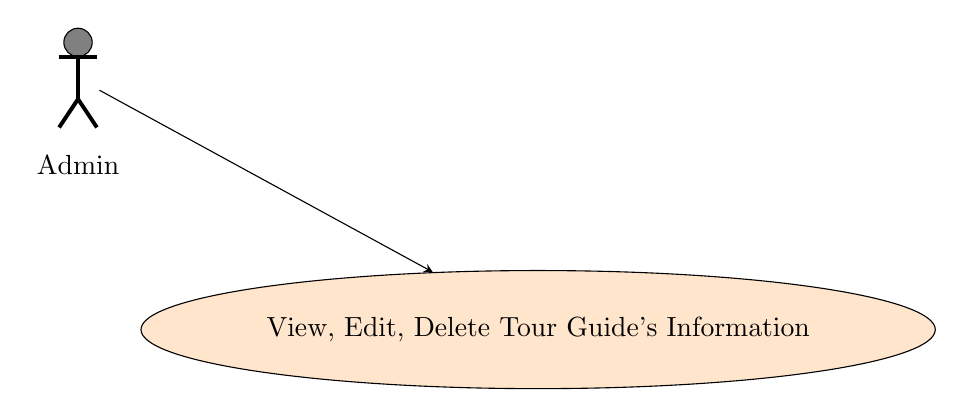
\begin{tikzpicture}[>=stealth]

            % Actor (Admin)
            \node[inner sep=0pt] (admin) at (0,0) {\tikz{\pic[scale=0.6] {stickman};}};
            \node[below=0.2cm of admin] {Admin};
        
            % Use Case with color
            \node[ellipse, draw, fill=orange!20, align=center, minimum width=6cm, minimum height=1.5cm, below right=2cm and 2cm of admin] (view) {View, Edit, Delete Tour Guide's Information};
        
            % Relationships
            \draw[->] (admin) -- (view);
        
        \end{tikzpicture}
    }
\end{center}
\begin{center}
    \parbox{0.8\textwidth}{ 
        \centering
        \textbf{Figure-7.8: Use Case 08}
    }
\end{center}

\paragraph {\textnormal{Brief Description: 
Admin manages the information of registered tour guides within the Odyssey Travels platform.}}

\subsection*{\textbf{Main Success Scenario:}}

\begin{enumerate}
    \item Admin logs into the Odyssey Travels admin dashboard.
    \item Navigates to "Manage Tour Guides" section.
    \item Views list of registered tour guides with their details.
    \item Selects a tour guide for viewing or editing.
    \item Reviews tour guide's information (contact details, certifications).
    \item Edits tour guide's information as required.
    \item Confirms changes and updates the tour guide's profile.
    \item Deletes tour guide's profile if necessary, after confirmation.
\end{enumerate}

\subsection*{\textbf{Postconditions:}}

\begin{itemize}
    \item Tour guide's information updated or deleted as per admin's actions.
    \item System reflects changes immediately.
\end{itemize}

\subsection*{\textbf{Alternative Courses:}}

\begin{itemize}
    \item Admin requests additional documentation or updates from the tour guide.
    \item Provides feedback or support regarding certification requirements.
\end{itemize}

\subsection*{\textbf{Exceptions:}}

\begin{itemize}
    \item Technical issues or system errors may delay updates.
    \item Admin decides to defer deletion due to ongoing bookings or other dependencies.
\end{itemize}

\section{Use Case Diagram}

A use case diagram is pivotal in illustrating a user's engagements with the system, depicting the correlation between the user and various use cases they engage in. This diagram serves to provide a comprehensive overview of the system and supports the detailed design process. The UML use case diagram comprises a collection of use cases that encompass all conceivable interactions outlined in the system requirements (Section 6). The use case diagram for Odyssey Travels is delineated in Figure-7.1.

\subsection *{ UML Diagram : }
{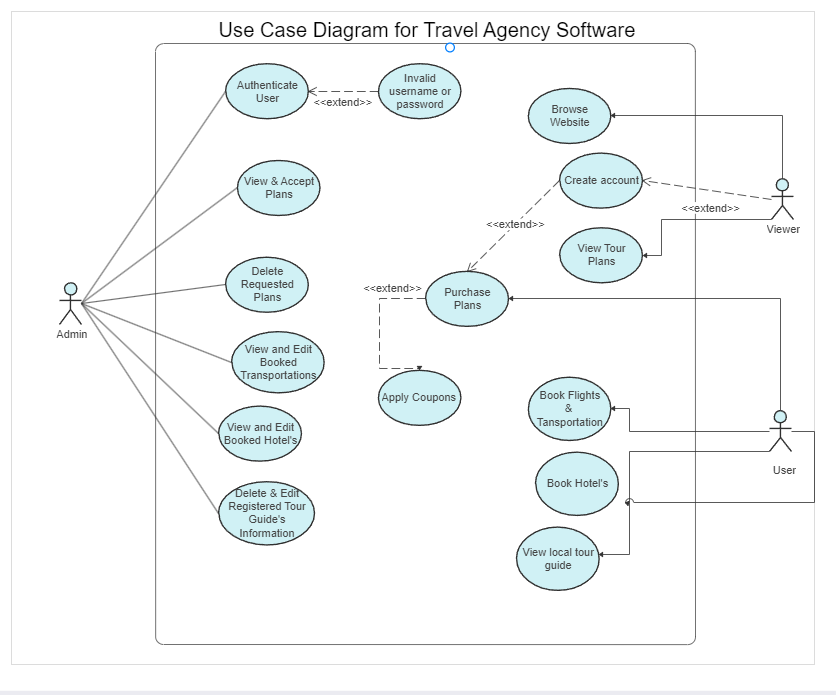
\includegraphics[width=450px, height=300px]{uml.png}}

\begin{center}
    \parbox{0.8\textwidth}{ 
        \centering
        \textbf{Figure - 7.9 : Use Case Diagram For Travel Agency Software}
    }
\end{center}

Although we adhere to the object-oriented approach (OOP) in developing our system, Data Flow Diagrams (DFDs) may occasionally be indispensable for enhanced comprehension. Therefore, we have included the DFDs of the Odyssey Travels project in Appendix-I to provide clarity where necessary.

\chapter{System Evolution}
We have formulated foundational assumptions pivotal for launching the Odyssey Travel Agency project. This section delineates these assumptions, addressing potential impacts from advancements in hardware/software, evolving user demands, and other pertinent factors.

Our software development lifecycle extends beyond initial deployment, encompassing ongoing refinement and adaptation. Post-deployment, adjustments may be necessary to address operational issues, accommodate platform updates, and enhance performance and other non-functional attributes. Given that our product is managed internally within our organization, ongoing support and evolution are integral to its lifecycle without necessitating additional contractual agreements.

The evolution process involves essential activities such as change analysis, release planning, system implementation, and customer delivery. We have identified potential post-deployment challenges and their underlying assumptions, summarized in Table-I, to proactively address and mitigate any arising issues.

\begin{center}
    \parbox{0.8\textwidth}{ 
        \centering
        \textbf{Table - I: Potential reasons that can cause severe problems during the evolution process of the travel website}
    }
\end{center}

\begin{table}[h!]
\centering
\begin{tabular}{|c|>{\raggedright\arraybackslash}p{13cm}|}
\hline
\textbf{SN.} & \textbf{Reasons that can drive us to make urgent changes} \\
\hline
1. & User encounters issues with booking confirmations not being received on time. Immediate action is required to fix the notification system to maintain customer trust. \\
\hline
2. & The integration with third-party services (e.g., flight or hotel booking APIs) changes their formats or access methods, causing disruptions in our service. We need to quickly adapt to these changes to keep our booking system functional. \\
\hline
3. & The website's performance degrades significantly under high traffic conditions, which can occur during peak travel seasons. We must improve the server scalability and optimize the codebase to handle increased loads effectively. \\
\hline
4. & New security vulnerabilities are discovered that could potentially expose user data. Immediate security patches and updates are necessary to protect user information and comply with data protection regulations. \\
\hline
5. & A major update is released for the mobile operating system that our mobile app relies on, leading to compatibility issues. We need to update the app promptly to ensure a seamless experience for our users. \\
\hline
\end{tabular}
\end{table}

\begin{center}
    \parbox{0.8\textwidth}{ 
        \centering
        \textbf{Table-II: Maintenance Predictions}
    }
\end{center}

\begin{table}[h!]
\centering
\begin{tabular}{|c|>{\raggedright\arraybackslash}p{8cm}|>{\raggedright\arraybackslash}p{4cm}|}
\hline
\textbf{SN.} & \textbf{Assumptions} & \textbf{Reengineering Technique} \\
\hline
1. & Interface updates will be necessary to accommodate new travel packages and user preferences. & Source code translation \\
\hline
2. & Certain requirements may change due to new regulations or changes in third-party services (e.g., new APIs for hotel bookings). & Program structure improvement \\
\hline
3. & As a new version is rolled out, a significant number of bug and failure reports can be expected due to the high variability in user environments. & Code refactoring \\
\hline
4. & Users may request specific feature enhancements such as multi-language support or personalized itinerary suggestions without needing a complete overhaul of the system. & Program modularization \\
\hline
5. & Integration with new social media platforms for sharing travel plans could require substantial backend modifications. & Integration and migration \\
\hline
\end{tabular}
\label{table:maintenance_predictions}
\end{table}

Maintenance Predictions for our travel website involve strategic planning to address potential challenges that could impact our system's functionality and user experience. One critical aspect is \textbf{source code translation}, where older programming languages are updated to newer versions or entirely different languages using automated tools, ensuring compatibility and performance enhancements. \textbf{Program structure improvement} is another vital strategy, focusing on analyzing and refining the control structures within our software to enhance readability and maintainability, often requiring a balance of automated tools and manual interventions. \textbf{Program modularization} plays a key role by organizing related components to streamline functionality and reduce redundancy, fostering easier updates and scalability. These techniques anticipate future needs, such as accommodating new travel packages and user preferences through interface updates. Additionally, they prepare us for regulatory changes or updates in third-party services, ensuring seamless integration and compliance. As we roll out new versions, addressing potential bugs and user environment variability becomes paramount, necessitating thorough \textbf{code refactoring} processes to optimize performance and stability. Finally, integrating with emerging social media platforms necessitates backend modifications, highlighting the importance of \textbf{integration and migration} strategies in our maintenance predictions. Overall, these proactive measures ensure our travel website remains robust, adaptable, and responsive to evolving customer demands and technological advancements.

\chapter{Appendix-I}
DFD (Data Flow Diagram) helps us understand the how the data is flowing across the system and
what is the relation between the functions of the system.
Level 0 DFD and Level 1 DFD of Efficiency Monitor are shown in figure-9.1 and figure-9.2
respectively.

\section{Level-0 Data Flow Diagram}



\begin{center}
    \parbox{0.8\textwidth}{ 
        \centering
        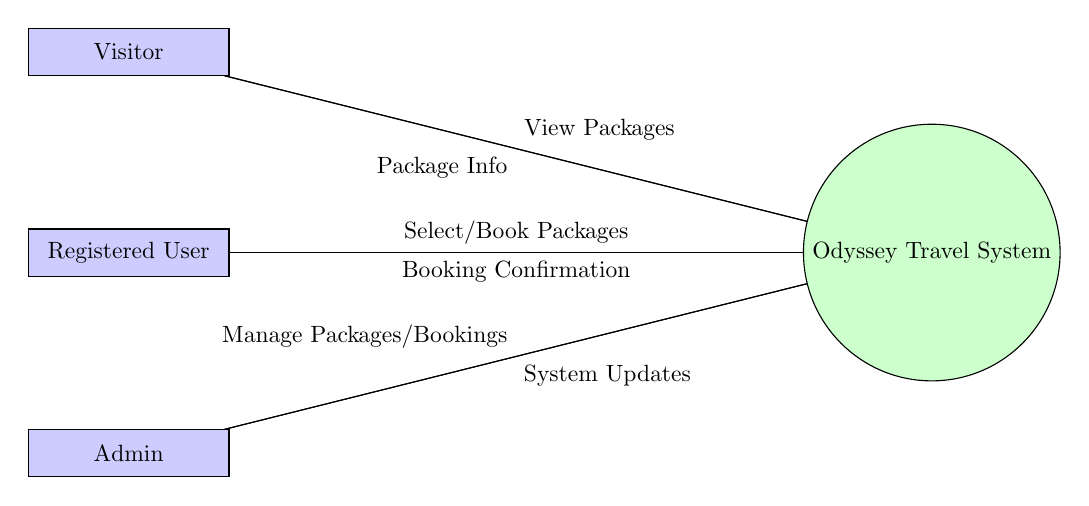
\begin{tikzpicture}[->,>=,auto,node distance=3cm,scale=0.85, transform shape]

            % Define styles
            \tikzstyle{external} = [rectangle, draw, fill=blue!20, text centered, minimum height=2em, minimum width=3cm]
            \tikzstyle{process} = [circle, draw, fill=green!20, text centered, minimum height=4em, minimum width=4em]
        
            % External Entities
            \node[external] (visitor) at (-6, 0) {Visitor};
            \node[external] (user) at (-6, -3) {Registered User};
            \node[external] (admin) at (-6, -6) {Admin};
        
            % Central Process
            \node[process] (system) at (6, -3) {Odyssey Travel System};
        
            % Data Flows
            \draw[->] (visitor) -- node[midway, midway] {View Packages} (system);
            \draw[->] (system) -- node[midway, midway] {Package Info} (visitor);
            \draw[->] (user) -- node[midway, midway] {Select/Book Packages} (system);
            \draw[->] (system) -- node[midway, below] {Booking Confirmation} (user);
            \draw[->] (admin) -- node[midway, midway] {Manage Packages/Bookings} (system);
            \draw[->] (system) -- node[midway, midway] {System Updates} (admin);
        
        \end{tikzpicture}
}
\end{center}

\begin{center}
    \parbox{0.8\textwidth}{ 
        \centering
        \textbf{Figure-9.1: Level 0 DFD of Travel Agency Software}
    }
\end{center}

\section{Level-1 Data Flow Diagram}

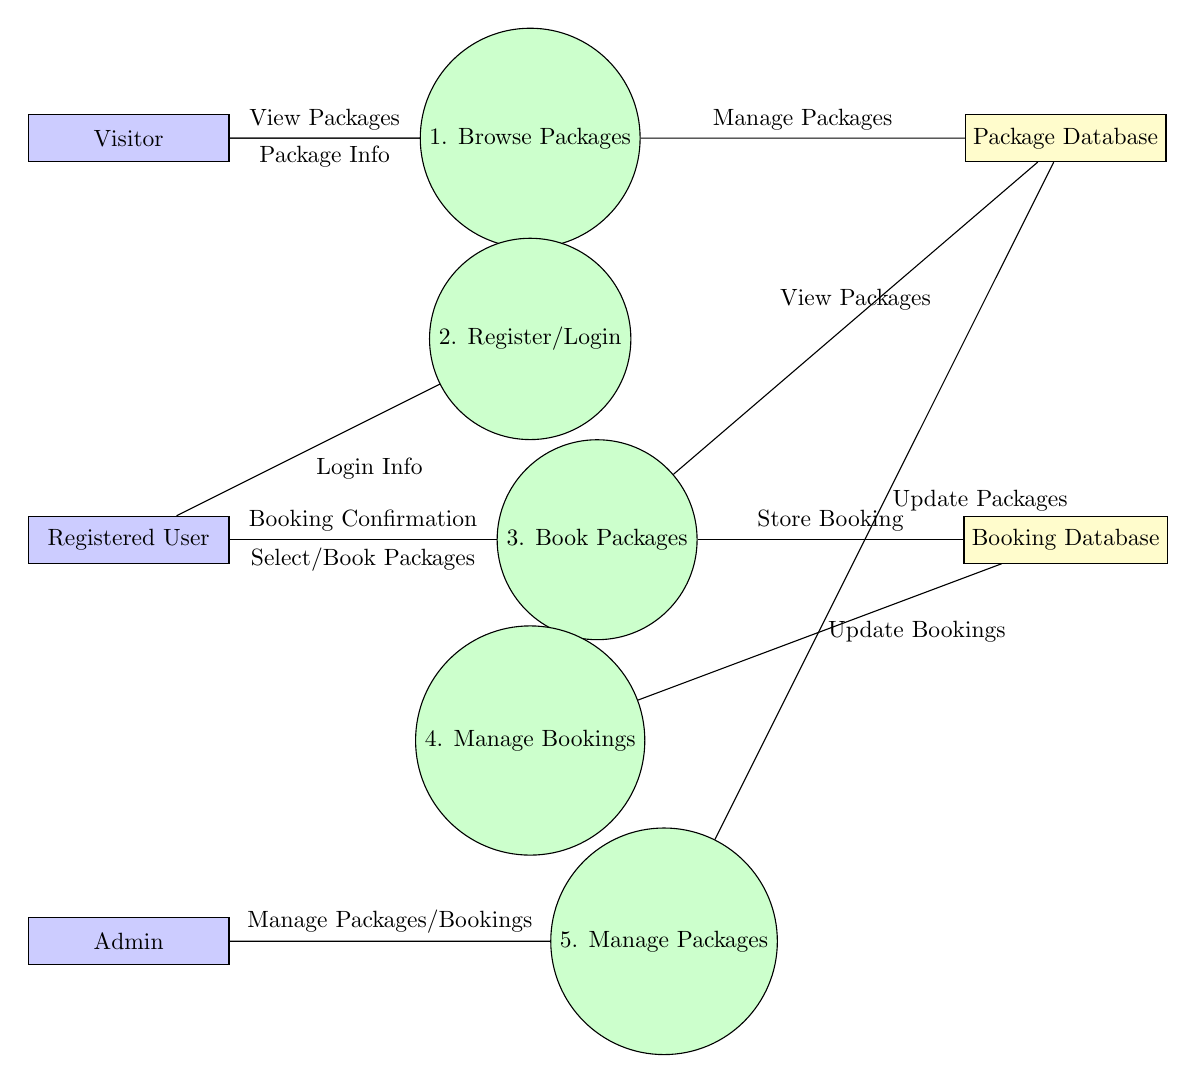
\begin{tikzpicture}[->,>=,auto,node distance=4cm,scale=0.85, transform shape]

    % Define styles
    \tikzstyle{external} = [rectangle, draw, fill=blue!20, text centered, minimum height=2em, minimum width=3cm]
    \tikzstyle{process} = [circle, draw, fill=green!20, text centered, minimum height=4em, minimum width=4em]
    \tikzstyle{data} = [rectangle, draw, fill=yellow!20, text centered, minimum height=2em, minimum width=3cm]

    % External Entities
    \node[external] (visitor) at (-6, 6) {Visitor};
    \node[external] (user) at (-6, 0) {Registered User};
    \node[external] (admin) at (-6, -6) {Admin};

    % Data Stores
    \node[data] (packageDB) at (8, 6) {Package Database};
    \node[data] (bookingDB) at (8, 0) {Booking Database};

    % Processes with serial numbers
    \node[process] (browse) at (0, 6) {1. Browse Packages};
    \node[process] (register) at (0, 3) {2. Register/Login};
    \node[process] (book) at (1, 0) {3. Book Packages};
    \node[process] (manageBooking) at (0, -3) {4. Manage Bookings};
    \node[process] (managePackage) at (2, -6) {5. Manage Packages};

    % Data Flows
    \draw[->] (visitor) -- node[midway, above] {View Packages} (browse);
    \draw[->] (browse) -- node[midway, below] {Package Info} (visitor);
    \draw[->] (browse) -- node[midway, above] {Manage Packages} (packageDB);

    \draw[->] (user) -- node[midway, below] {Select/Book Packages} (book);
    \draw[->] (book) -- node[midway, above] {Booking Confirmation} (user);
    \draw[->] (book) -- node[midway, above] {Store Booking} (bookingDB);
    \draw[->] (book) -- node[midway, above] {View Packages} (packageDB);

    \draw[->] (admin) -- node[midway, above] {Manage Packages/Bookings} (managePackage);
    \draw[->] (managePackage) -- node[midway, right] {Update Packages} (packageDB);
    \draw[->] (manageBooking) -- node[midway, right] {Update Bookings} (bookingDB);

    \draw[->] (register) -- node[midway, midway] {Login Info} (user);

\end{tikzpicture}

\begin{center}
    \parbox{0.8\textwidth}{ 
        \centering
        \textbf{Figure-9.2: Level 1 DFD of Travel Agency Software}
    }
\end{center}


\section*{Conclussion}
The Odyssey Travel Agency project is poised to The Odyssey Travel Agency project aims to simplify and enhance the way people plan and manage their travels. Our platform makes it easy for users to book flights, hotels, and tour guides through a user-friendly interface, ensuring a smooth and enjoyable experience. With real-time updates and secure transactions, users can confidently organize their trips, whether it's for a quick getaway or an extended adventure. We also provide personalized recommendations and support for applying discounts, making travel planning more affordable and efficient. As we continue to develop our platform. Our goal is to make Odyssey Travel Agency a reliable and helpful tool that travelers can depend on for all their journey needs.
\end{document}